\documentclass[journal]{IEEEtran}

% Packages
\usepackage{cite}
\usepackage{graphicx}
\usepackage{float}
\usepackage{stfloats}
\usepackage{amsmath, amssymb}

\begin{document}

% Title
\title{Role of dispersion relation effect in topological surface-enhanced Raman scattering
}

% Author Information
\author{Wenqi Ji
\thanks{Wenqi Ji is with Department of Electrical and Computer Engineering, Rice University, Houston, USA (email: wj28@rice.edu).}
}

% Make title
\maketitle

% Abstract
\begin{abstract}
Raman spectroscopy provides molecular fingerprint information through inelastic light scattering, but its intrinsically weak signal limits trace-level detection. Surface-enhanced Raman scattering (SERS) addresses this limitation through both electromagnetic enhancement from localized near fields and chemical enhancement associated with interfacial charge transfer. Recent studies suggest that topological materials, especially Weyl semimetals, may offer new opportunities for Raman enhancement because their unusual band structures and surface states can modify optical response and promote charge transfer. In this project, we investigate topological surface-enhanced Raman scattering by designing nanostructured hybrid stacks combining noble metals with topological materials. COMSOL simulations, Raman measurements, and optical characterization are used to analyze electric-field enhancement, resonance behavior, and optical responses relevant to Raman enhancement. We expect the new stack design to approximately double Raman enhancement.
\end{abstract}
% Introduction
\section{Introduction}
\indent
Raman spectroscopy is a powerful technique for probing vibrational and rotational modes through the inelastic scattering of monochromatic laser light by a material. The energy difference between the incident and scattered photons, known as the Raman shift, serves as a molecular fingerprint and gives rise to the Stokes and anti-Stokes lines, thereby enabling chemical identification and structural characterization. However, the intrinsic Raman signal is typically very weak because of the inherently small Raman cross-section. Although Raman spectroscopy provides rich information on chemical composition and molecular structure and is widely used in materials and chemical analysis, trace-level detection still requires effective strategies to enhance the Raman signal\cite{doi:10.1021/acs.jpclett.9b01146}.\\
\indent
Surface-enhanced Raman scattering (SERS) has therefore emerged as a powerful analytical technique because of its exceptional sensitivity for trace detection\cite{doi:10.1021/acs.jpclett.5c01197}. The enhancement in SERS is generally attributed to two mechanisms: the electromagnetic mechanism (EM) and the chemical mechanism (CM)\cite{doi:10.1021/acs.jpclett.5c01197}. The EM mechanism mainly arises from localized surface plasmon resonance (LSPR) in plasmonic nanostructures, as illustrated in Fig.~\ref{fig:Raman enhancement}(a). Under optical excitation, collective oscillations of free electrons generate highly localized electromagnetic fields near the nanostructure surface, thereby substantially amplifying the Raman signal. In this case, the enhancement factor is commonly approximated to scale with the fourth power of the local electric field, namely $|E|^{4}$\cite{https://doi.org/10.1002/advs.202302568,Yi2016}.\\
\indent
In addition to electromagnetic enhancement, Raman signals can also be amplified through the chemical mechanism, which mainly originates from charge transfer (CT) between the substrate and the adsorbed molecule, as illustrated in Fig.~\ref{fig:Raman enhancement}(b). Such interfacial electronic coupling can modify the molecular electron density and enhance molecular polarizability, thereby increasing the Raman scattering efficiency\cite{CONG2020100051}.\\
\indent
Recently, topological materials have attracted increasing attention in photonic and optoelectronic research because their nontrivial band topology can give rise to unusual electronic and optical responses, as well as strong light--matter interactions. Among them, Weyl semimetals are characterized by discrete band-crossing points in momentum space, known as Weyl nodes\cite{Guo2023}. Their unique electronic structures provide new opportunities for tailoring optical responses and promoting interfacial charge-transfer processes.\\
\indent
As shown in Fig.~\ref{fig:Raman enhancement}(b), charge-transfer-induced Raman enhancement can occur in both conventional metallic substrates and topological materials. In conventional metallic substrates with parabolic band dispersion, Raman enhancement may arise from charge transfer between the molecule and the substrate. In contrast, topological materials with linear band dispersion, such as Weyl or Dirac semimetals, may facilitate more efficient interfacial charge transfer because of their unique electronic structures and surface states, thereby strengthening the CM contribution to Raman scattering\cite{HOU2021100488}.\\
\begin{figure}[H]
\centering
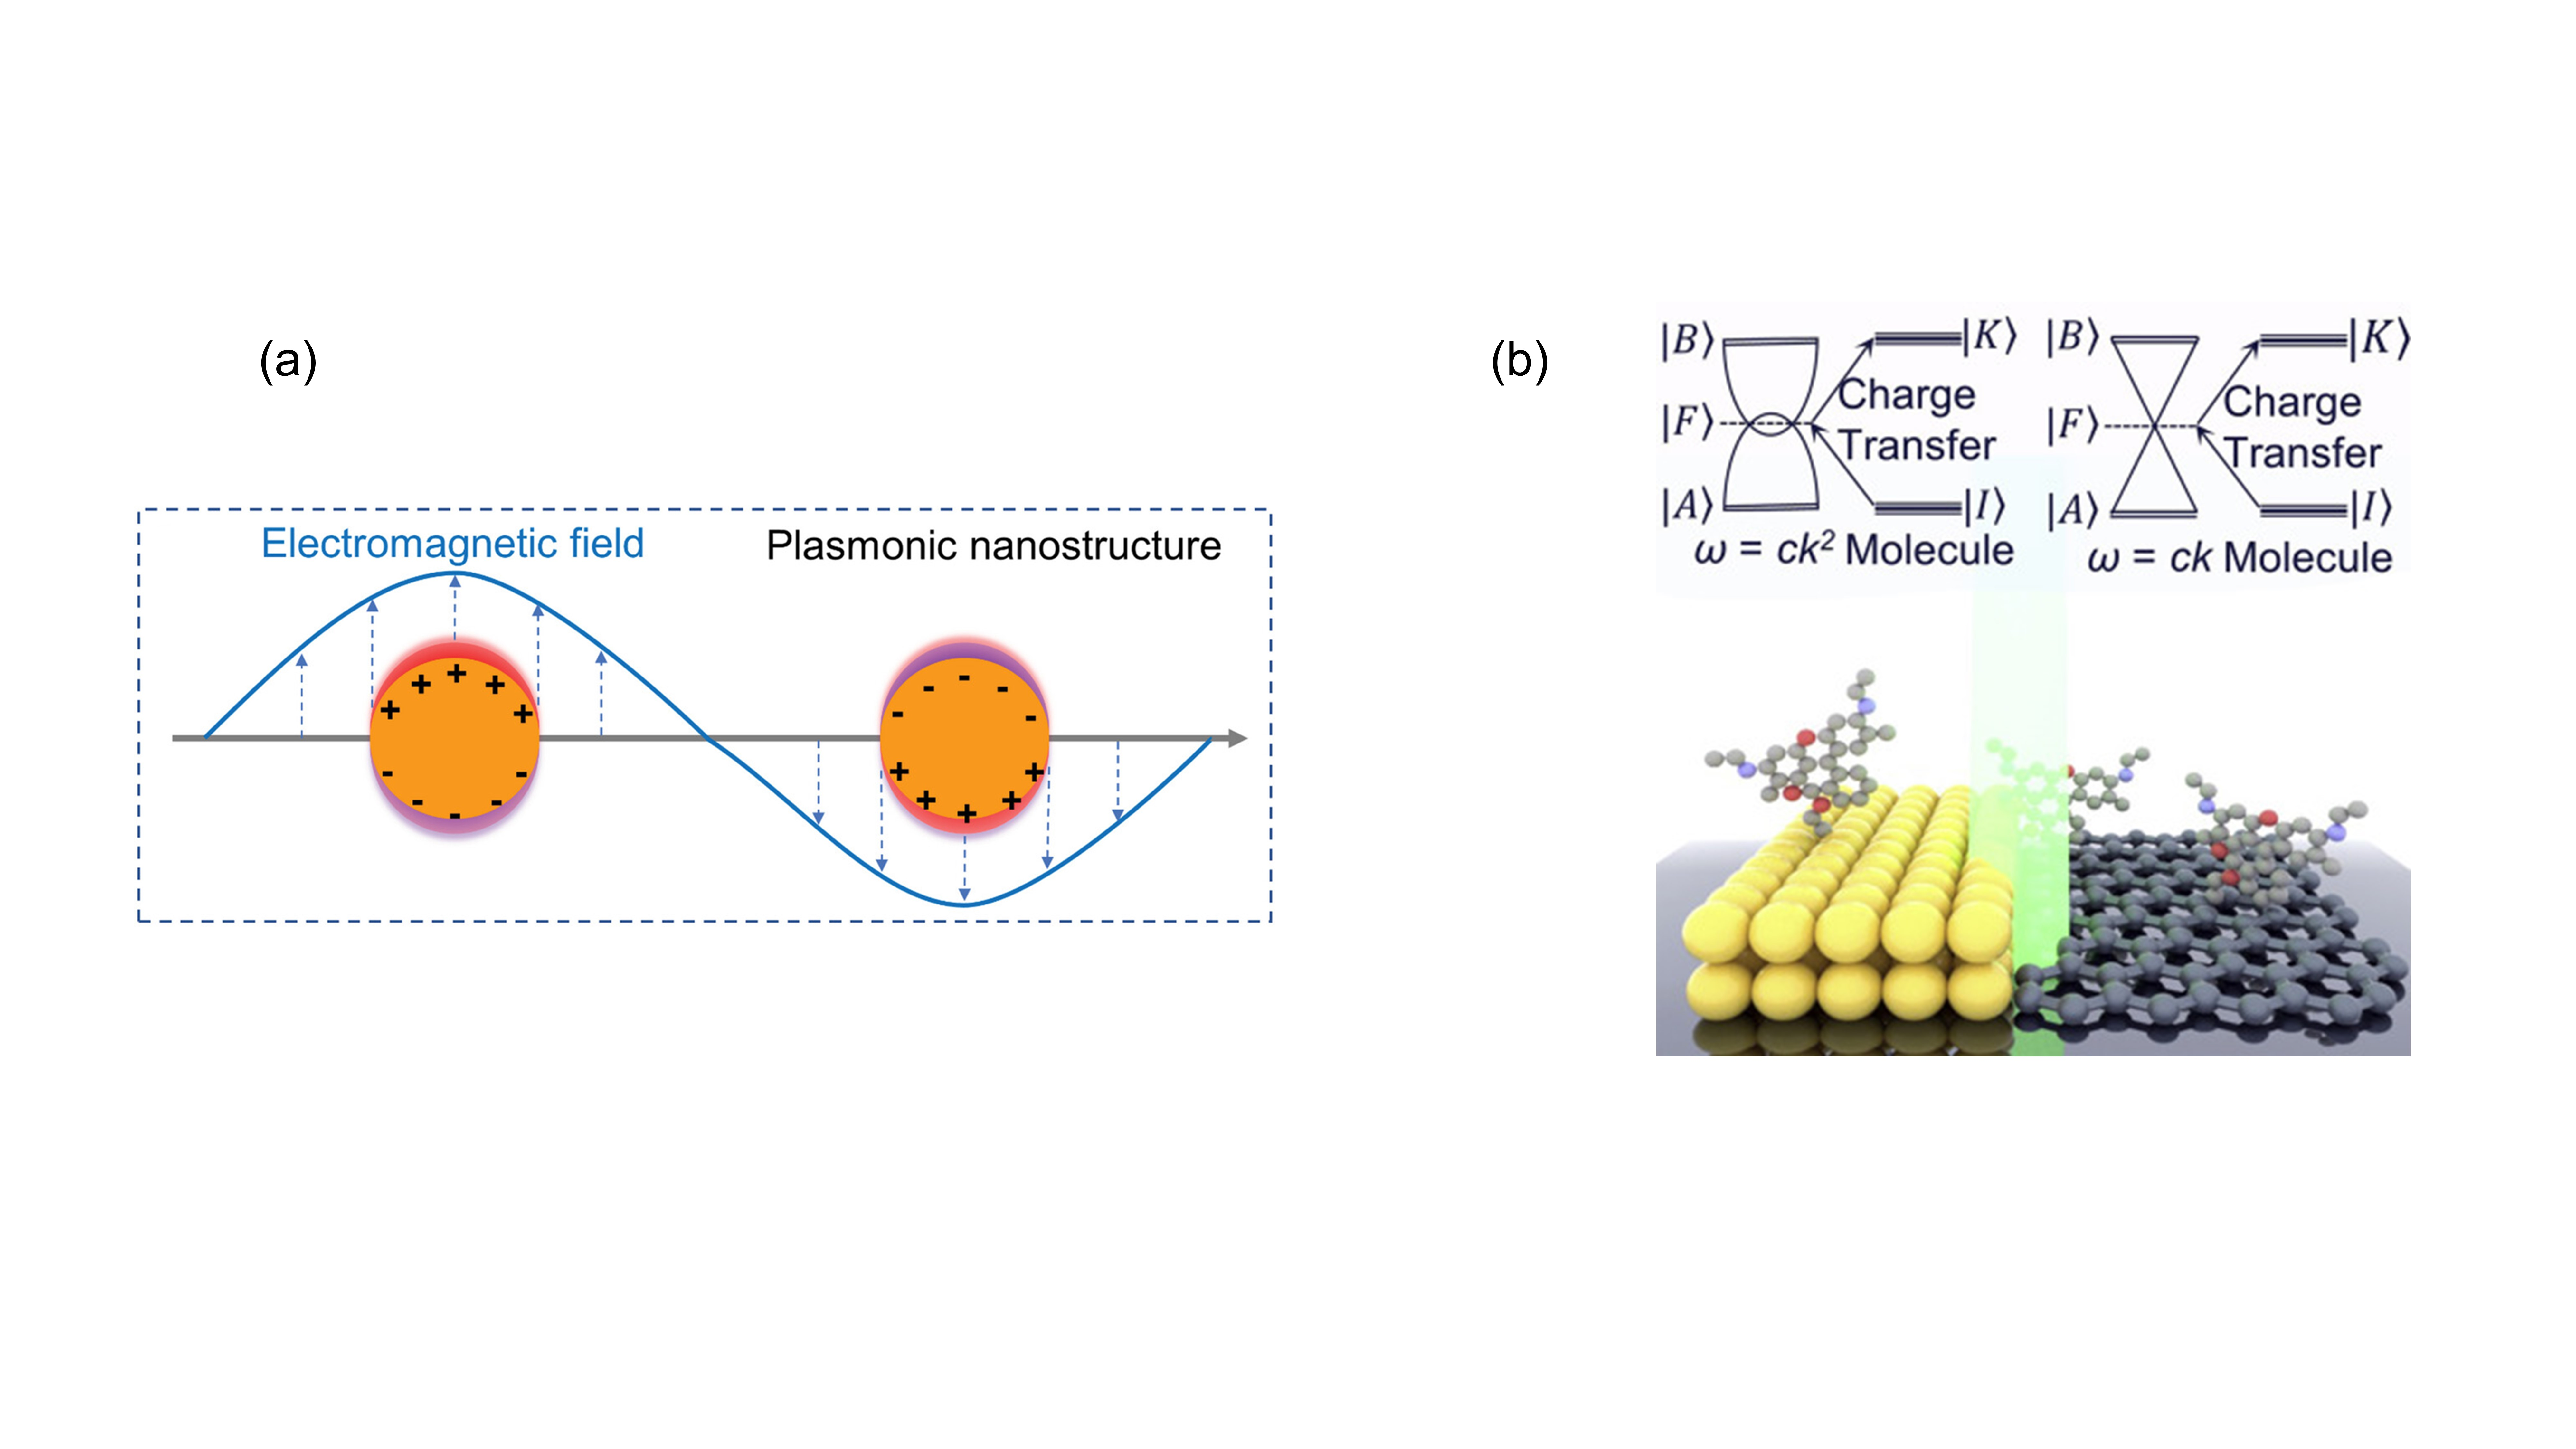
\includegraphics[width=80mm]{Raman enhancement.jpg}
\caption{(a) Schematic illustration of localized surface plasmon resonance (LSPR) in a plasmonic nanostructure\cite{https://doi.org/10.1002/advs.202302568}. 
(b) Schematic illustration of Raman enhancement via charge transfer\cite{HOU2021100488}.
} 
\label{fig:Raman enhancement} 
\end{figure}
\indent
Recent theoretical studies have shown that Weyl semimetals can host unusual surface plasmonic modes associated with their topological surface states, indicating their potential for strong light-matter interaction and plasmonic applications\cite{7b1l-gkjy}. When nanostructured, Weyl semimetals may further support surface or localized plasmonic modes similar to those in noble metals. These near-field modes can enhance the local electric field and may consequently contribute to Raman signal enhancement for molecules near the surface. Such findings motivate the exploration of nanostructured Weyl semimetals for localized field enhancement and Raman-related applications.\\
\indent
Among these materials, Co$_2$MnGa, a magnetic topological semimetal in the Heusler family, has demonstrated promising electronic, magnetic, and optical properties\cite{Swekis2021}. These characteristics suggest that Co$_2$MnGa may serve as a promising material platform for Raman-related and nanophotonic applications.\\
\indent
Because topological surface states and finite-thickness effects can contribute to the optical response, they may modify the effective optical constants of the material, particularly in thin or nanostructured samples. Therefore, thin films of topological materials may exhibit optical constants ($n$ and $k$) that deviate from those of the corresponding bulk material\cite{Xu2022,FANG2020144822}.\\
\indent
To further support the optical analysis of topological-material-based Raman enhancement platforms, ellipsometry and micro-reflectance spectroscopy with a CCD detector were performed on WTe$_2$ to characterize its bulk optical constants and thin-layer reflectance spectra. These measurements provide experimental optical parameters for comparison with transfer-matrix-method calculations and help clarify the optical response relevant to Raman enhancement.

% Methods
\section{Methods}
\indent
Electromagnetic simulations were performed in COMSOL Multiphysics to evaluate the near-field enhancement at the Co$_2$MnGa surface for both the actual sample geometry and an idealized periodic model.\\
\indent
For the actual sample, the simulation model was constructed as shown in Fig. \ref{fig:comsol actual}(a), consisting of an upper air layer and a lower Co$_2$MnGa layer, both with thicknesses of several micrometers. Perfectly matched layers were applied at the top and bottom boundaries to eliminate spurious reflections. Electromagnetic simulations were performed using the Electromagnetic Waves, Frequency Domain (ewfd) module in COMSOL Multiphysics, with a downward-propagating plane wave incident from the top boundary. The rough interfacial profile in the central region of the model was obtained from atomic force microscopy (AFM) measurements of the actual sample surface. And to account for the 2 nm thick gold layer deposited on the Co$_2$MnGa surface, the gold film was modeled using a transition boundary condition rather than an explicit geometric layer, due to the surface roughness of the sample and the limited computational memory available for the simulation.\\
\indent
For the idealized model, a periodic nanohole array was established, as illustrated in Fig.~\ref{fig:comsol nanohole}(a). Key geometric parameters, including the hole depth and lattice period, were systematically varied to identify the configuration that maximized the electric-field enhancement. Perfectly matched layers with a thickness of 900 nm were introduced at the top and bottom boundaries, while periodic boundary conditions were applied to the lateral boundaries of the computational domain. Simulations were also performed using the Electromagnetic Waves, Frequency Domain (ewfd) module in COMSOL Multiphysics, with a downward-propagating plane wave launched from the top boundary as the background excitation field.\\
\indent
In addition to introducing a thin gold layer on the top surface, a Drude material layer was also considered in the idealized model, since the permittivity of gold is close to that of Co$_2$MnGa in the investigated spectral range. The relative permittivity of the Drude material is expressed as shown in Eq. \ref{eq:Drude}.\\
\begin{equation}
\varepsilon_r=\varepsilon_{\infty}-\frac{\omega_p^2}{(2\pi f)^2+i\gamma(2\pi f)}
\label{eq:Drude}
\end{equation}
\indent
where $\varepsilon_{\infty}$ is the high-frequency dielectric constant, $\omega_p$ is the plasma frequency, $\gamma$ is the damping constant, and $f$ is the frequency of the incident electromagnetic wave.\\
\indent
The initial Drude parameters were chosen as $\varepsilon_{\infty}=1$, $\omega_p=1.66\times10^{16}~\mathrm{s}^{-1}$, and $\gamma=1.44\times10^{14}~\mathrm{s}^{-1}$. The corresponding simulation results are presented in Fig.~\ref{fig:comsol nanohole}. Furthermore, $\gamma$ and $\omega_p$ were systematically swept while $\varepsilon_{\infty}$ was kept constant.\\
\indent
For the optical constants of the other materials in the simulations, the Co$_2$MnGa data were taken from our own measurements, whereas the optical constants of gold were adopted from the default material data provided in COMSOL, which are based on the experimental results of Johnson and Christy.\\
% Results
\section{Results}
\indent
Fig. \ref{fig:comsol actual} shows the geometric model and simulated results for part of the actual Co$_2$MnGa sample. The electric field enhancement is mainly concentrated around the nanostructured scratches, corresponding to regions with negative surface height in the $z$ direction. The simulated enhancement pattern is broadly consistent with the measured Raman mapping results. Nevertheless, a one-to-one spatial correspondence is not expected, since the Raman signal is collected over a finite laser spot of approximately 1~$\mu$m in diameter, which limits the spatial resolution and leads to spatial averaging of the local response.\\
\begin{figure}[H]
\centering
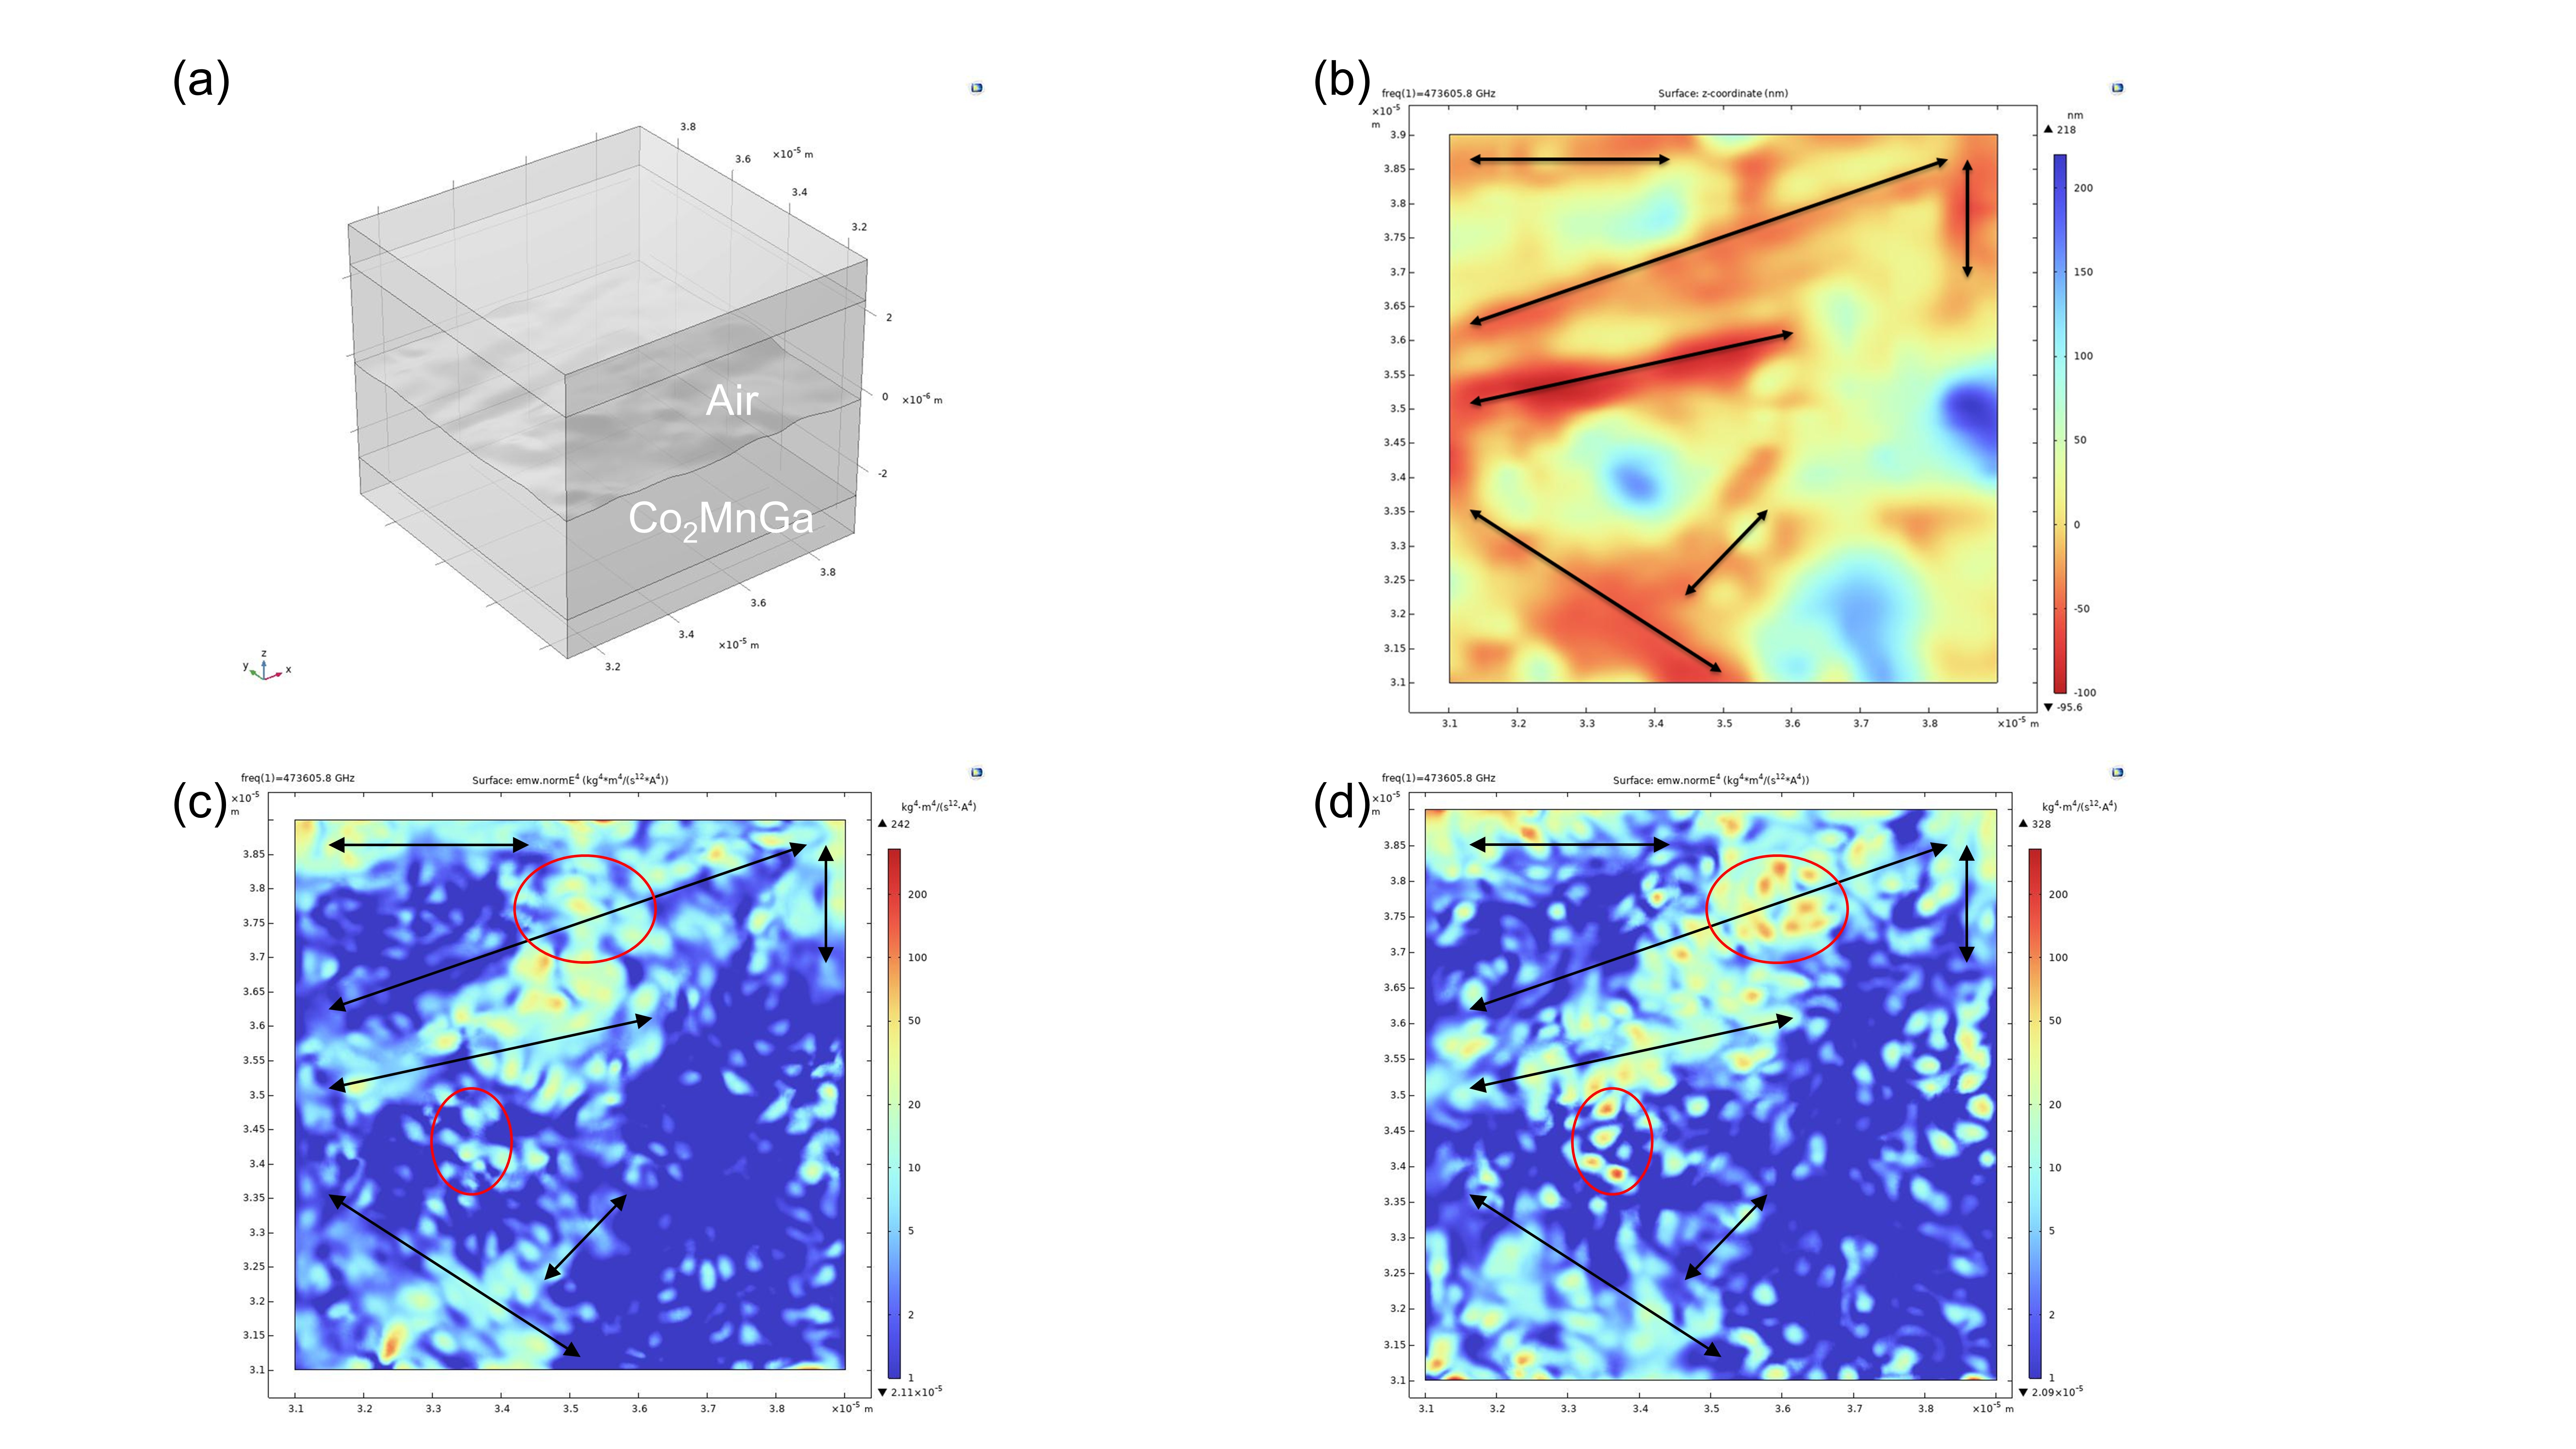
\includegraphics[width=80mm]{comsol actual.jpg}
\caption{(a) Geometric model of the actual Co$_2$MnGa sample. (b) Surface height map of the rough Co$_2$MnGa surface in the $z$ direction. (c) Simulated electric field enhancement on the surface of the actual Co$_2$MnGa sample. (d) Simulated electric field enhancement on the surface of the 2 nm Au layer coated on the actual Co$_2$MnGa sample. The black lines indicate nanostructured scratches on the sample surface, while the red circles highlight regions where the electric field is noticeably enhanced after coating with the 2 nm Au layer.
} 
\label{fig:comsol actual} 
\end{figure}
\indent
Since the simulation results for the actual Co$_2$MnGa sample did not permit a sufficiently clear conclusion, an idealized periodic Co$_2$MnGa nanohole model was further constructed, as shown in Fig. \ref{fig:comsol nanohole}. Both the non-semicircular and semicircular nanohole geometries exhibit their maximum electric field at a nanohole depth of approximately 110 nm, in good agreement with the Raman enhancement measurements. Furthermore, for the non-semicircular nanohole geometry, the introduction of a gold layer or a Drude layer leads to more pronounced localized enhancement, whereas such selective enhancement is much less apparent in the semicircular case. In addition, the non-semicircular geometry maintains a higher overall electric field intensity than the semicircular geometry throughout the entire nanohole-depth sweep.\\
\indent
\begin{figure}[H]
\centering
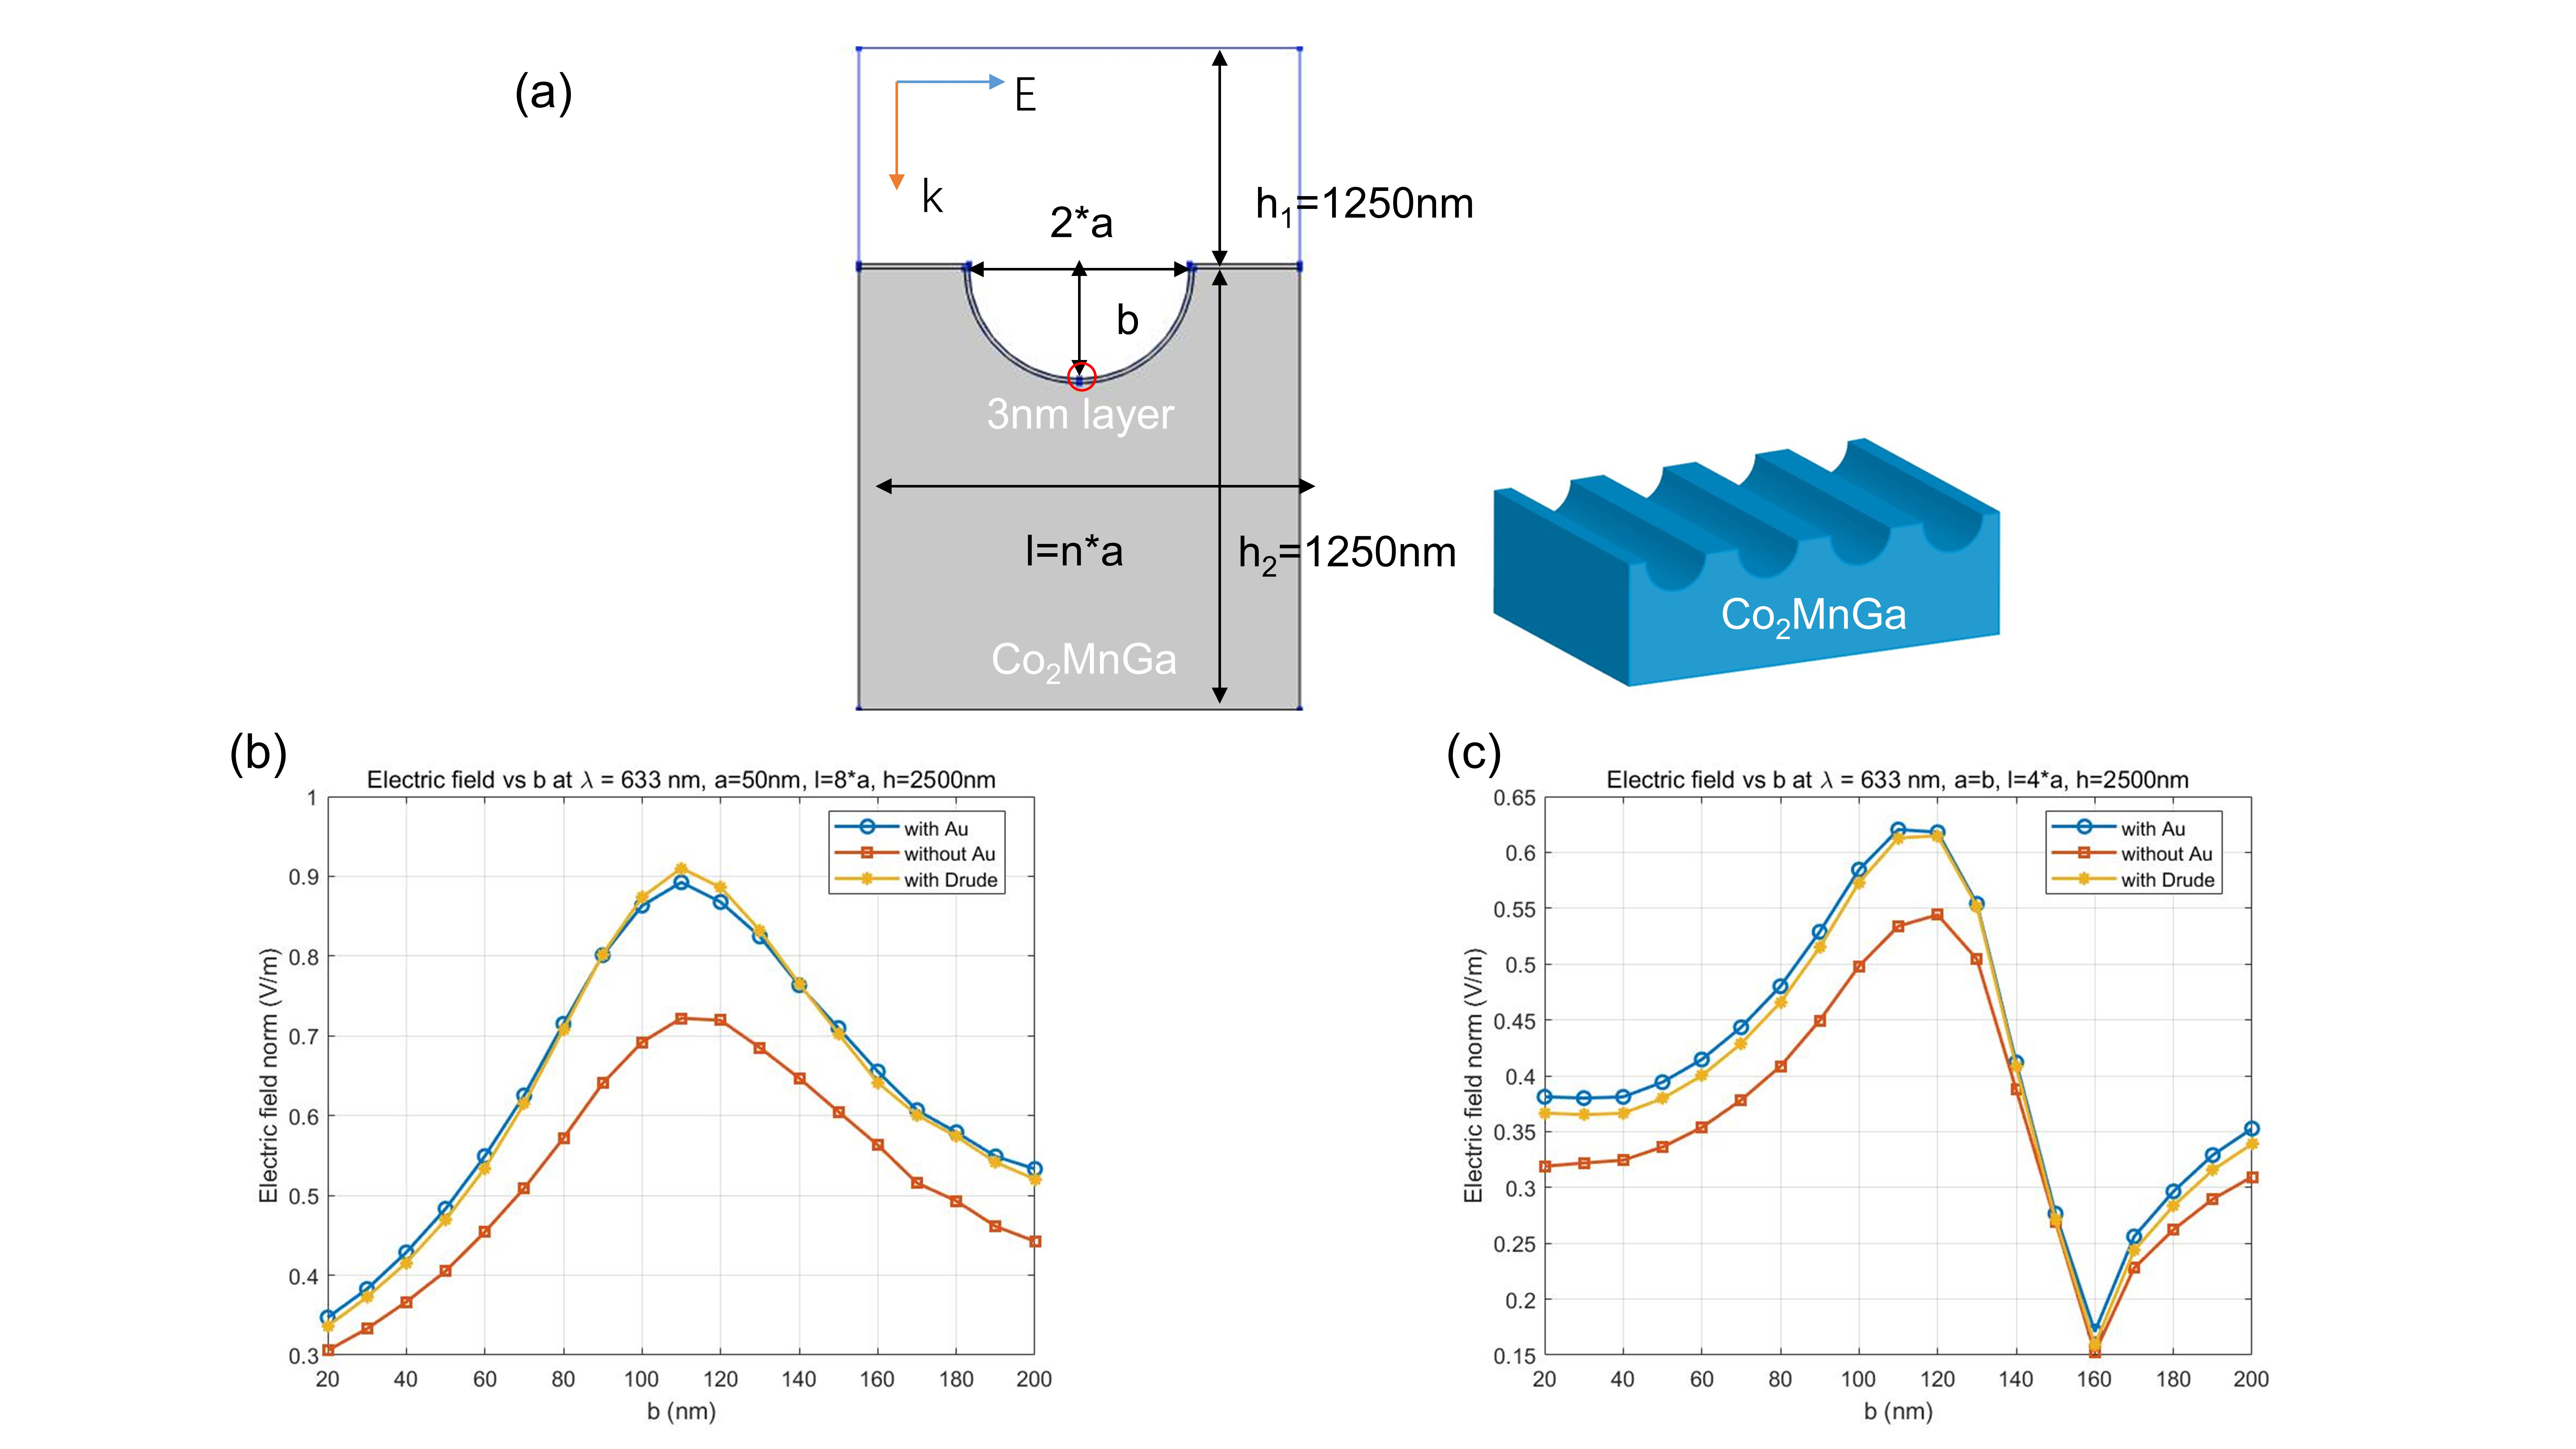
\includegraphics[width=80mm]{comsol nanohole.jpg}
\caption{(a) Geometric model of the idealized periodic Co$_2$MnGa nanohole structure. The total height is defined as $h=h_1+h_2$. The red circle indicates the bottom center of the nanohole, where the electric field is evaluated. (b) Electric field magnitude at the bottom center of the nanohole as a function of nanohole depth $b$ for a fixed $a$, corresponding to a generally non-semicircular hole profile ($a\neq b$). (c) Electric field magnitude at the bottom center of the nanohole as a function of nanohole depth $b$ for the case of $a=b$, where the hole profile remains semicircular. In both (b) and (c), the results for bare Co$_2$MnGa and for structures with a 3 nm Au or Drude layer are compared.
} 
\label{fig:comsol nanohole} 
\end{figure}
\indent
Since the initial Drude parameters selected for the Drude layer did not lead to obvious changes in the results presented in Fig.~\ref{fig:comsol nanohole}, a systematic parameter sweep of $\gamma$ and $\omega_p$ around the initial value was carried out while $\varepsilon_{\infty}$ was kept fixed. The corresponding electric field values obtained from the swept Drude parameters are presented below.\\
% Discussion
\section{Discussion}
\indent
The current results suggest that surface morphology plays an important role in determining the local electric-field enhancement on Co$_2$MnGa-based structures. For the actual sample, the simulated hotspots are mainly concentrated near scratched or depressed regions of the rough surface, which is broadly consistent with the Raman mapping trend. However, a strict one-to-one correspondence is not expected because the Raman signal is collected over a finite laser spot, which spatially averages the local response. Therefore, the actual-sample model is useful for identifying qualitative enhancement trends, but it is less suitable for isolating the individual effects of geometry and material response.\\
\indent
The idealized periodic nanohole model provides a clearer picture of the geometry dependence. Both the non-semicircular and semicircular structures show maximum field enhancement at a nanohole depth of around 110 nm, in agreement with the Raman measurements. In addition, the non-semicircular geometry exhibits both stronger overall enhancement and a more pronounced response to the added a gold or Drude layer. These results indicate that geometric asymmetry and local curvature may be important factors for concentrating the electromagnetic field in this platform.\\
% Acknowledgements
\section*{Acknowledgements}
I would like to thank Prof. Shengxi Huang and Xielin Wang for their invaluable guidance and support throughout this project. ChatGPT was used for language polishing, including grammar correction and improvement of clarity and flow.\\
\section*{CRediT Author Statement}
Wenqi Ji: Conceptualization, Methodology, Investigation, Formal analysis, Visualization, Writing.\\
% References
\bibliographystyle{IEEEtran}
\bibliography{references}

\end{document}